\documentclass[aspectratio=169,professionalfonts]{beamer}

\usepackage[utf8]{inputenc}
\usepackage[T1]{fontenc}
\usepackage{graphicx}
\usepackage{booktabs}
\usepackage{array}
\usepackage{listings}
\usepackage{xcolor}

\usetheme{Madrid}
\usecolortheme{default}
\setbeamertemplate{navigation symbols}{}
\setbeamertemplate{footline}[frame number]

\definecolor{qriscblue}{RGB}{40,82,130}
\definecolor{qriscgray}{RGB}{245,247,250}
\setbeamercolor{structure}{fg=qriscblue}
\setbeamercolor{frametitle}{fg=white,bg=qriscblue}
\setbeamercolor{title}{fg=white,bg=qriscblue}

\lstdefinestyle{qrisc-code}{
  basicstyle=\ttfamily\small,
  keywordstyle=\color{qriscblue}\bfseries,
  commentstyle=\color{gray},
  backgroundcolor=\color{qriscgray},
  frame=single,
  framerule=0.2pt,
  columns=fullflexible,
  keepspaces=true,
  showstringspaces=false
}
\lstset{style=qrisc-code}

\newcommand{\bits}[1]{\texttt{#1}}
\newcommand{\fieldtable}[2]{%
  \begin{center}
  \resizebox{\textwidth}{!}{%
  \begin{tabular}{>{\centering\arraybackslash}p{0.13\textwidth}%
                  >{\centering\arraybackslash}p{0.12\textwidth}%
                  >{\centering\arraybackslash}p{0.08\textwidth}%
                  >{\centering\arraybackslash}p{0.13\textwidth}%
                  >{\centering\arraybackslash}p{0.11\textwidth}%
                  >{\centering\arraybackslash}p{0.12\textwidth}%
                  >{\centering\arraybackslash}p{0.12\textwidth}%
                  >{\centering\arraybackslash}p{0.12\textwidth}}
  \toprule
  #1\\
  \midrule
  #2\\
  \bottomrule
  \end{tabular}}
  \end{center}
}

\title{Qrisc32}
\subtitle{Five-stage RISC CPU}
\author{Viacheslav Vinogradov}
\date{Converted from \texttt{risc\_present.odp}}

\begin{document}

\begin{frame}
  \titlepage
  \begin{itemize}
    \item 5-stage RISC.
    \item AXI4-style instruction read master.
    \item AXI4-style data read/write master.
    \item 32 general-purpose 32-bit registers.
    \item Two EX-stage flags: Zero and Carry.
  \end{itemize}
\end{frame}

\begin{frame}{Instruction Set}
  \begin{itemize}
    \item Unconditional load to register.
    \item Unconditional store from register to memory.
    \item Unconditional jumps.
    \item Conditional relative jumps.
    \item ALU commands.
    \item Conditional load to register.
  \end{itemize}
\end{frame}

\begin{frame}{Instruction Fetch Stage}
  \begin{columns}[T,totalwidth=\textwidth]
    \begin{column}{0.55\textwidth}
      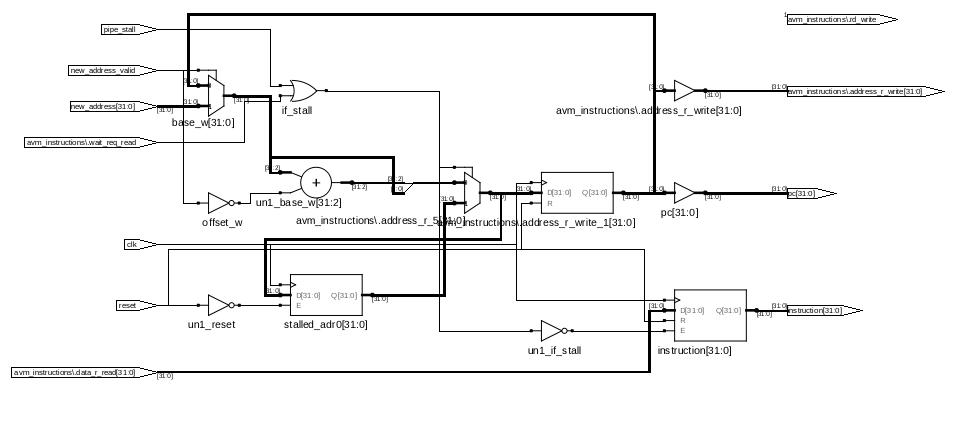
\includegraphics[width=\linewidth,height=0.68\textheight,keepaspectratio]{risc_present_assets/if_stage.jpg}
    \end{column}
    \begin{column}{0.4\textwidth}
      \begin{itemize}
        \item Fetches instruction words from memory.
        \item Changes the program counter.
        \item Transfers PC value to the next stage for CALL and RETURN commands.
      \end{itemize}
    \end{column}
  \end{columns}
\end{frame}

\begin{frame}{Instruction Decode Stage}
  \begin{itemize}
    \item Decodes instruction words.
    \item Activates control signals for the next stage.
    \item Reads values from the register file.
    \item Contains the writeback stage.
    \item Writeback stores register values from the EX and MEM stages.
  \end{itemize}
\end{frame}

\begin{frame}{Execution Stage}
  \begin{itemize}
    \item Executes operations according to ID-stage control signals.
    \item Changes the SRC2 register by -4, -2, -1, 0, 1, 2, or 4.
    \item Forwards results to writeback and can bypass the MEM stage.
  \end{itemize}
\end{frame}

\begin{frame}{Memory Stage}
  \begin{itemize}
    \item Reads and writes memory.
    \item Contains an internal pipeline for AXI-style memory requests.
    \item Current repo contract uses single-beat, 32-bit aligned transfers.
    \item Read and write stages wait for their corresponding bus responses.
  \end{itemize}
\end{frame}

\begin{frame}{Forwarding}
  \begin{itemize}
    \item EX stage forwards results to the ID stage.
    \item Writeback can write from two sources: EX/DST and MEM/DST or MEM/SRC2.
    \item ID can obtain register values from EX, MEM, or the register file.
  \end{itemize}
\end{frame}

\begin{frame}{Branch Taken}
  \begin{itemize}
    \item Branch-taken cost is 4 cycles.
    \item Advantage: simple IF stage.
    \item Disadvantage: large zero-slot delay.
    \item Efficient programs must account for the branch delay.
  \end{itemize}
\end{frame}

\begin{frame}{Instruction Format: LDR}
  \fieldtable
    {\bits{31:28} & \bits{27:26} & \bits{25} & \bits{24:22} & \bits{21:15} & \bits{14:10} & \bits{9:5} & \bits{4:0}}
    {LDR & type & off & incr src2 & reserved & src2 & src1 & dst}
  \begin{itemize}
    \item Type 0: \texttt{Rdst = Rsrc1}.
    \item Type 1: \texttt{Rdst[31:16] = code[20:5]} (\texttt{LDRH}).
    \item Type 2: \texttt{Rdst[15:0] = code[20:5]} (\texttt{LDRL}).
    \item Type 3: \texttt{Rdst = [Rsrc1 + offset]}.
  \end{itemize}
\end{frame}

\begin{frame}{Instruction Format: STR}
  \fieldtable
    {\bits{31:28} & \bits{27:26} & \bits{25} & \bits{24:22} & \bits{21:15} & \bits{14:10} & \bits{9:5} & \bits{4:0}}
    {STR & type & off & incr src2 & reserved & src2 & src1 & dst}
  \begin{itemize}
    \item Stores \texttt{Rdst} to \texttt{[Rsrc1 + offset]}.
    \item Syntax: \texttt{STR Rdst, [Rsrc1 + offset], INCR2}.
  \end{itemize}
\end{frame}

\begin{frame}{Instruction Format: Unconditional Jumps}
  \fieldtable
    {\bits{31:28} & \bits{27:26} & \bits{25} & \bits{24:22} & \bits{21:15} & \bits{14:10} & \bits{9:5} & \bits{4:0}}
    {JMP & type & off & offset/incr & code & src2 & src1 & dst}
  \begin{itemize}
    \item Type 0: \texttt{pc[25:0] = code[25:0]}.
    \item Type 1: \texttt{pc = pc + offset}.
    \item Type 2: \texttt{pc = pc + offset}, \texttt{Rdst = pc}.
    \item Type 3: \texttt{pc = Rdst}.
  \end{itemize}
\end{frame}

\begin{frame}{Instruction Format: Conditional Jumps}
  \fieldtable
    {\bits{31:28} & \bits{27:26} & \bits{25} & \bits{24:22} & \bits{21:15} & \bits{14:10} & \bits{9:5} & \bits{4:0}}
    {JMPF & cond & off & offset & reserved & src2 & src1 & dst}
  \begin{itemize}
    \item Type 0: \texttt{JMPZ pc = pc + offset}.
    \item Type 1: \texttt{JMPNZ pc = pc + offset}.
    \item Type 2: \texttt{JMPC pc = pc + offset}.
    \item Type 3: \texttt{JMPNC pc = pc + offset}.
  \end{itemize}
\end{frame}

\begin{frame}{Instruction Format: ALU}
  \fieldtable
    {\bits{31:28} & \bits{27:25} & \bits{24:22} & \bits{21:15} & \bits{14:10} & \bits{9:5} & \bits{4:0} &}
    {ALU & op & incr src2 & reserved & src2 & src1 & dst &}
  \begin{itemize}
    \item 0: AND, 1: OR, 2: XOR, 3: ADD.
    \item 4: MUL, 5: shift left, 6: shift right, 7: compare.
  \end{itemize}
\end{frame}

\begin{frame}{Instruction Format: Conditional Load}
  \fieldtable
    {\bits{31:28} & \bits{27:26} & \bits{25} & \bits{24:22} & \bits{21:15} & \bits{14:10} & \bits{9:5} & \bits{4:0}}
    {LDRF & cond & off & incr src2 & reserved & src2 & src1 & dst}
  \begin{itemize}
    \item 0: \texttt{LDRZ Rdst = Rsrc1} if Z is set, otherwise \texttt{Rsrc2}.
    \item 1: \texttt{LDRNZ Rdst = Rsrc1} if Z is clear, otherwise \texttt{Rsrc2}.
    \item 2: \texttt{LDRC Rdst = Rsrc1} if C is set, otherwise \texttt{Rsrc2}.
    \item 3: \texttt{LDRNC Rdst = Rsrc1} if C is clear, otherwise \texttt{Rsrc2}.
  \end{itemize}
\end{frame}

\begin{frame}{Common Instruction Fields}
  \fieldtable
    {\bits{31:28} & \bits{27:26} & \bits{25} & \bits{24:22} & \bits{21:15} & \bits{14:10} & \bits{9:5} & \bits{4:0}}
    {opcode & type & off & incr src2 & code/off & src2 & src1 & dst}
  \begin{itemize}
    \item DST is the register that receives the operation result.
    \item SRC1 and SRC2 provide operation inputs.
    \item INCR SRC2 changes SRC2 by -4, -2, -1, 0, 1, 2, or 4.
    \item Off selects offset source: immediate code or signed SRC2.
  \end{itemize}
\end{frame}

\begin{frame}{Sorting Algorithms}
  \begin{itemize}
    \item Shell sort.
    \item Modified shell sort.
    \item Bubble sort.
    \item Test data contains 10 integer words.
  \end{itemize}
\end{frame}

\begin{frame}[fragile]{Shell Sort}
\begin{lstlisting}[language=C]
ShellSort(int *a) {
  int inc, i, j, temp;
  for (inc = 5; inc > 0; inc = inc / 2) {
    for (i = inc; i < 10; i += 1) {
      temp = a[i];
      for (j = i; (j >= inc) && (a[j-inc] > temp); j -= inc) {
        a[j] = a[j-inc];
      }
      a[j] = temp;
    }
  }
}
\end{lstlisting}
\end{frame}

\begin{frame}[fragile]{Modified Shell Sort}
\begin{lstlisting}[language=C]
for (inc = 20; inc > 0; inc = inc / 2) {
  for (i = inc; i < 40; i += 4) {
    temp = a[i];
    for (j = i; (j >= inc) && (a[j-inc] > temp); j = j - inc) {
      a[j] = a[j-inc];
    }
    a[j] = temp;
  }
}
\end{lstlisting}
\end{frame}

\begin{frame}[fragile]{Bubble Sort}
\begin{lstlisting}
R0 = mem[00]; R1 = mem[04]; R2 = mem[08]; R3 = mem[0c]; R4 = mem[10];
R5 = mem[14]; R6 = mem[18]; R7 = mem[1c]; R8 = mem[20]; R9 = mem[24];

R10 = R0;
R11 = R0; // minimum
if R1 < R11 then R11 = R1;
...
if R9 < R11 then R11 = R9;
mem[0] = R11;
\end{lstlisting}
\end{frame}

\begin{frame}{Sorting Performance}
  \begin{tabular}{lccc}
    \toprule
    Algorithm & Reverse & Random & Sorted\\
    \midrule
    Shell & 842 & 612 & 176\\
    Modified shell & 712 & 669 & 519\\
    Bubble & 455 & 455 & 455\\
    \bottomrule
  \end{tabular}
  \vspace{1em}
  \begin{itemize}
    \item Average cycles from the original slide: shell 543, modified shell 633, bubble 455.
    \item Bubble sort has the most stable runtime for this 10-word test.
  \end{itemize}
\end{frame}

\end{document}
